\section{Аналитический метод}

Вывод программы решения игры аналитическим методом представлена на
рисунке~\ref{fig:fig1}.

\begin{figure}
  \centering
  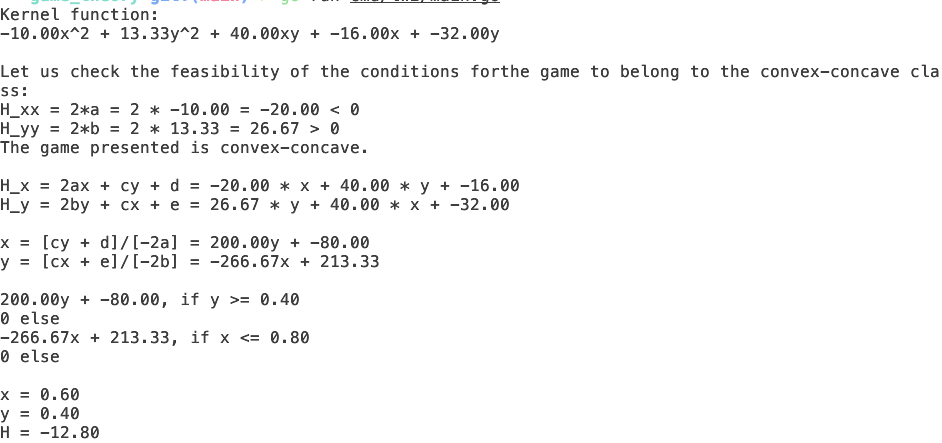
\includegraphics[scale=0.5]{../../artifacts/lw2/analytical.png}
  \caption{Решение выпукло-вогнутой игры аналитическим методом}
  \label{fig:fig1}
\end{figure}


Функция выигрыша имеет вид:
\[
H(x,y) = -10x^2 + \frac{40}{3}y^2 + 40xy - 16x - 32y.
\]
При этом
\[
\frac{\partial^2 H}{\partial x^2} = -20 < 0, \quad \frac{\partial^2 H}{\partial y^2} = \frac{80}{3} > 0,
\]
то есть функция ковогнута по \(x\) и выпукла по \(y\), что подтверждает принадлежность игры к классу выпукло-ковогнутых.

Равновесная точка \((x,y)\) определяется решением системы условий первого порядка:
\[
\frac{\partial H}{\partial x}=0,\quad \frac{\partial H}{\partial y}=0.
\]

Путём решения системы были найдены оптимальные стратегии игроков:
\[
x = 0{,}6, \quad y = 0{,}4,
\]
при которых значение функции выигрыша (цена игры) составляет:
\[
H(x, y) = -12{,}8.
\]
